\section{Introduction}
\label{sec:intro}

\subsection{Motivation}
%\begin{itemize}
%	\item Motivate Software engineering and QA during software engineering.
%	\item Motivate Commit Validation as method to reduce engineering costs.
%	\item Shortly mention some Commit Validation approaches as examples (CLEVER \cite{Nayrolles2018}, CommitGuru \cite{Rosen2015}, maybe Kamei? \cite{Kamei2013}).
%	\item Background of the problem
%\end{itemize}

Software quality belongs to the many relevant topics of software engineering, one which often directly maps to costs and expenses. While good quality leads to well-maintainable code and reduced effort, software faults can lead to very expensive results. The US National Institute of Standards and Technology has estimated that software faults and failures cost the US economy \$59.5 billion a year \cite{nist,Rosen2015}.

Typical approaches focus on analyzing module artifacts such as files or packages and attempt to detect faults in those. However, this often introduces additional problems. Kamei et al. reported on typical drawbacks such as the fact that it is hard to find a responsible expert for an identified faulty code location as development teams tend to become large for large-scale projects, and that just identifying a faulty package still leaves much effort for the developer to find the actual code location of the fault \cite{Kamei2013}. Finally, a primary problem is that typical approaches find faults only very late during the development cycle, which is much more expensive than fixing them early \cite{Martin08}.

A recent approach for increasing software quality and thus decreasing costs is the concept of Commit Validation. This concept is used at a very technical level where change commits on software projects are automatically analyzed and verified in regards to the probability that they introduce a new software fault. This is much more efficient because code is analyzed for faults at an early phase when the responsible developer is still involved with the changes. \cite{Kamei2013}

Different approaches exist on this topic,
%There exist different approaches on this topic, 
one of the early works was made as a study on the topic by Kamei et. al. which was based on Just-in-Time Bug Detection on commit data \cite{Kamei2013}. Similar approaches were introduced by Yang and Rosen by introducing approaches called \textit{Deeper} and \textit{Commit Guru} respectively \cite{Yang2015,Rosen2015}. Goyal introduced a concept based on the rating of abnormality of commits, called \textit{Unusual Commits} \cite{Goyal2017}. Finally, one of the most recent approaches was introduced by Nayrolles et. al. as \textit{CLEVER}, which not only detected buggy commits, but also automatically suggested code fixes \cite{Nayrolles2018}. This paper will focus on these five approaches in more detail.

\subsection{Problem Definition}
%\begin{itemize}
%	\item Discuss the Problem Definition of this work
%	\begin{itemize}
%		\item Describe the problems that motivate existing approaches.
%		\item Describe the goals that this paper tries to fulfill and discuss how it realizes a solution for these goals.
%		\item State the success criteria for this work.
%	\end{itemize}
%\end{itemize}

Apart from just these five approaches, there exist many more different tools with varying techniques on the topic of Commit Validation.
%There exists different tools with varying techniques on the topic of Commit Validation. 
As this is an emerging topic with many published works in the past few years, a clear State of the Art approach has not been defined yet, and it is hard to choose a suitable Commit Validation technique for a new project to leverage its benefits. 

The goal of this paper is to explore how Commit Validation techniques can be compared in an objective way, and to define a method for choosing a fitting Commit Validation technique for a Software Engineering project.

To satisfy this goal the paper will propose an objective evaluation scheme to compare existing Commit Validation techniques in an objective and fair way. Then a selection of five recent relevant technical approaches will be compared using the proposed evaluation scheme in an effort to give guidelines for determining which approaches are suitable in which context. These five approaches are described in sections \ref{sec:searchprocess} and \ref{sec:comparison}.

%TODO
%The following success criteria have been defined for this paper: 
%\begin{itemize}
%	\item The proposed comparison scheme does not take any considerations into account that are not relevant for Commit Validation approaches.
%	\item The proposed comparison scheme takes the context for which the compared approaches were designed for into account.
%	\item The comparison result of the compared approaches is specified in an explanatory way that helps potential readers to see for which use case the approach is suitable for.
%	\item The paper serves as guidelines for readers to find a suitable Commit Validation technique for their use cases.
%\end{itemize}

For this paper, four success criteria have been defined: 
(1) The proposed comparison scheme does not take any considerations into account that are not relevant for Commit Validation approaches;
(2) The 
%proposed comparison 
scheme takes the context for which the compared approaches were designed into account;
(3) The comparison result of the compared approaches is specified in an explanatory way that helps potential readers recognize for which use case the approach is suitable; and
(4) The paper serves as guidelines for readers to find a suitable Commit Validation technique for their use cases.

%  When working with commit based Version Management Systems, manual effort and costs can be significantly reduced by leveraging methods of automated Fault Prediction and Fault Prevention. As this is an emerging topic with many published works in the past few years, a clear State of the Art approach has not been defined yet. The goal of this work is to introduce the reader to the concept of commit validation, introduce 5 relevant approaches that have been implemented and compare them with an evaluation scheme that will be proposed. The evaluation scheme should compare the approaches in fair way to give insights to their effectiveness and use cases.


\subsection{Scope of This Paper}
\label{sec:scope}

%\begin{itemize}
%	\item Describe which kinds of work have been considered for this paper.
%	\item Describe why naive commit-checking techniques such as just "tests are green, coverage is high enough, sonarqube gates passed" have not been considered.
%	\item Discuss why works based on fault-detection unrelated to commits have not been considered for this paper.
%\end{itemize}

This paper focuses on Just-in-Time Fault Detection approaches which have the concept of code commits in mind. 
While the research area for code quality is large, the focus restricts the area into a limited set of research works.

The Just-in-Time aspect and the relevance of commits is important to fight the aforementioned drawback of typical code quality approaches, which is the expensiveness of fixing bugs much later after they were introduced into the project. 
There exist various approaches which just focus on detecting bugs and generating fixes such as Getafix by Bader et. al. or iFixR by Koyuncu et. al., however they are out of scope for this paper as the commit concept is not considered \cite{Bader2019,Koyuncu2019}.


\subsection{Outline}
This section gives an introduction on the topic and a problem definition and scope for this paper.

Section \ref{sec:background} introduces the background of Commit Validation, Just-in-Time Fault Detection and -Prevention as well as statistical measures which were used during the performance comparison.

Section \ref{sec:comparingapproaches} specifies how Commit Validation approaches can be compared, while the following section \ref{sec:comparison} describes the results from the comparison on the five selected approaches. A discussion of the results follows in section \ref{sec:discussion}.

The paper ends with an overview of related surveys on the topic in section \ref{sec:relatedsurveys} and the concluding section \ref{sec:conclusions}.

%\begin{itemize}
%	\item Describe the outline of this work.
%\end{itemize}


\section{Background on Commit Validation}
\label{sec:background}

This chapter introduces the topic of Commit Validation. 
First, a description of the process of Commit Validation, its target, and how it is implemented in a developers workflow is given, 
%First the process of Commit Validation, its target and how it is implemented in a developers workflow is described, 
then its two major components, Just-in-Time Fault Detection and Just-in-Time Fault Prevention are specified. Finally some statistical measures are explained which will be used later in this paper for comparing the methods' performances.


\subsection{Commit Validation Process}
\label{sec:cvprocess}

%\begin{itemize}
%	\item Introduce the basics on Commit-based QA.
%	\item Outline how Commit Validation is implemented in a developers workflow.
%\end{itemize}

%%TODO in a previous chapter, define "Commit Validation" and other names that are used in literature, and maybe that this name is specifically used for this paper

There are many ways of increasing software quality in the field of software engineering. While the field is very broad, there are many tools and technical utilities that have been established as part of a state-of-the-art technology stack. Among others, that also includes \define{version-control systems}{VCS}. A version-control system is used to track the evolution of source code and enables collaborative teams of software developers to cooperate on a consistent code base \cite{Chacon:2014:PG:2695634}. Currently, the most used VCS is \textit{Git}. %TODO cite 

An important concept for VCS are \textit{commits}, small sets of code changes that usually happen atomically and are annotated by the developer describing what the changes do. Commits are explicitly performed by the developer and usually mark a finished feature, bug-fix, chore work or similar artifacts. Because of that, the time at which a developer performs a commit is a suitable time for validating the change and analyzing it to find potential bugs that have been introduced while the developer still has the changes in his mind, yet considers them to be final. %TODO citation?

Git supports a concept called \textit{Hooks}. A hook specifies a custom script which runs programmatically in response to an event such as commits or uploading a set of commits to a remote server (which is called a \textit{Push} event). 
Git distinguishes between \textit{Client-Side Hooks}, which run on the local device of the developer that is authoring the commit, and \textit{Server-Side Hooks}, which run on the remote server \cite{Chacon:2014:PG:2695634}.
%Such hooks are differentiated into \textit{Client-Side Hooks}, which run on the local device of the developer that is authoring the commit, and \textit{Server-Side Hooks}, which run on the remote server. \cite{Chacon:2014:PG:2695634}

A variety of approaches exist
%There exists a variety of approaches 
for analyzing the quality of code changes at commit time. A popular approach is the manual authoring of unit-, integration- or end-to-end-tests to verify that a project's implementation fulfills its specification \cite{Maayan2018}. Such test definitions can be setup as a commit hook for them to run at commit time.

However, this paper focuses on approaches which do not require manual specifications such as test cases to detect a faulty commit, but instead automatically rate the probability of a commit to introduce a bug by leveraging external data sources that are available.
While such typical approaches like manual test cases come with extra effort and other drawbacks, a primary disadvantage over more automatized methods like Fault Detection becomes clear with the well known quote by Dijkstra: "Testing shows the presence, not the absence of bugs!" \cite{JohnN1969}.

A concluding overview of the typical commit validation process is shown in figure \ref{fig:cvprocess}. As detailed, the process starts either in response to the precommit hook directly after the commit process or to the push hook after a set of commits was pushed to a remote server. Then, the commit changesets are usually used to extract metrical vectors which in turn are used to classify the commit data as faulty or not.

\begin{figure}[t]
	\centering
	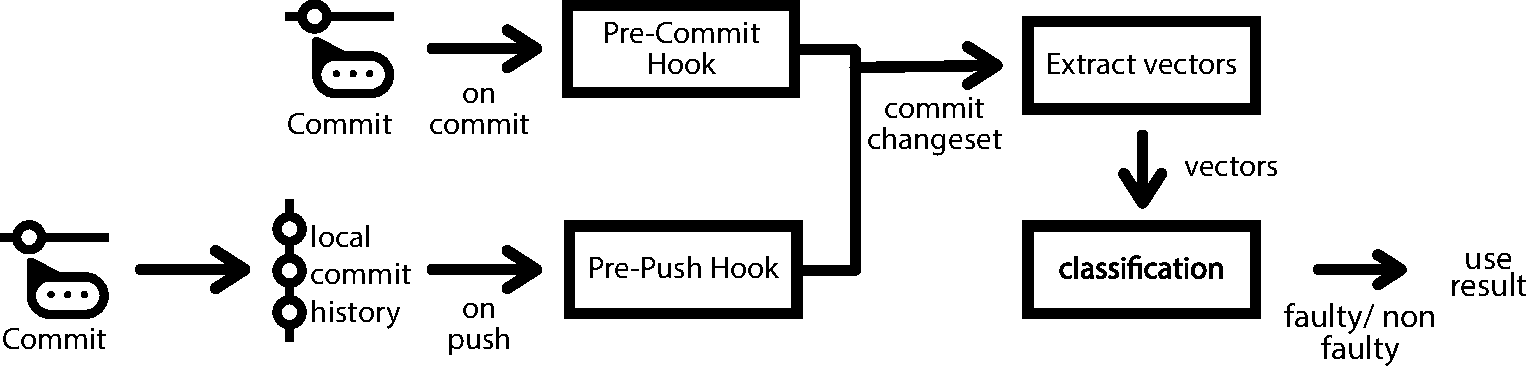
\includegraphics[width=\textwidth]{images/commitvalidation-process/typicalprocess-pdf}
	\caption{The typical commit validation process.}
	\label{fig:cvprocess}
\end{figure}

\subsection{Just-In-Time Fault Detection}
%TODO (TODO: Some of these subsections might have to be moved to section \ref{sec:cvprocess})
%\begin{itemize}
	%\item Introduce Just-in-Time Fault Detection.
	%TODO\item Discuss why Just-in-Time Fault Detection is necessary and how it benefits developers.
	%\item Showcase how a potentially "faulty" commit looks like (unusually big, commits at unusual times, touching rarely touched files, see \cite{Goyal2017}).
	%\item Describe how bug-tracking/issue-tracking systems can be used to gather data about bug-introducing commits and matching bugfix-commits.
	%TODO\item Describe how this can be implemented using static metrics extracted from commits.
	%TODO\item Describe how this can be implemented using pattern recognition on commits.
%\end{itemize}

While it may seem to be uncomplicated to hook analysis events to commit-based VCS, the actual analysis of commits to determine whether they are faulty or not, i.e. whether they introduce a bug which was not part of the system before, is a much more complicated task~\cite{Nayrolles2018, Kamei2013}. This procedure is referred to as \textit{Just-In-Time Fault Detection}.

When trying to identify potentially faulty commits, there are many metrics and characteristics that can be taken into account. Typical metrics include how many lines of code were added, removed or changed in a commit, characteristics about the developer, or the time of day during which the commit happened~\cite{Goyal2017}. There are various motivations which justify these metrics, such as the fact that developers who commit during a late time are likely to implement a last-minute bug-fix that could not wait until the next day, and thus are more likely to introduce new bugs in commits made under time pressure.

%There are more complex methods of detecting a faulty commit as described in~[TODO reference].

When validating a new commit, it has to be matched against some kind of database or it has to be evaluated with a model trained with a training dataset. Thus, an important part of Fault Detection is the data source from where this training or matching information comes. Usually the past commit data of the project is used as training data.
%Rosen et. al. also stated that enough time had to be elapsed since a commit for it to be taken as training data in form of a faulty example commit such that it had a chance to be fixed by a follow-up commit \cite{Rosen2015}.
This data needs to be labeled for bugs so that it can be used to train the bug detection model.
%There exist various ways
Various ways
of extracting labels for commit data exist, like using external issue systems which associate issue reports and bug-introducing commits.
%This leads to the second part of the required data, information which identifies the past commit data as either faulty or not. 

%TODO evtl absatz ebenfalls woanderst einbringen oder (eher das:) umformulieren sodass die 5 ansätze nicht so stark referenziert werden und es nicht als vergleich rüberkommt
%TODO absatz noch nicht proofread
%When validating a new commit, it has to be matched against some kind of database or it has to be evaluated with a model trained with a training dataset. Thus, an important part of Fault Detection is the data source from where this training or matching information comes from. The approaches that were identified in this paper all used the commit histories of the analyzed project as raw data source. In the work of Nayrolles et. al. even the commit histories of similar projects were taken into account \cite{Nayrolles2018}. 
%Rosen et. al. also stated that enough time had to be elapsed since a commit for it to be taken as training data in form of a faulty example commit such that it had a chance to be fixed by a follow-up commit \cite{Rosen2015}.
%This leads to the second part of the required data, information which identifies the past commit data as either faulty or not. 

% TODO!!! diesen absatz woanderst reinbringen...
%TODO absatz noch nicht proofread
%Three of the five considered approaches took external issue systems into account (\cite{Nayrolles2018, Yang2015, Kamei2013}). A issue system, or bug tracker, is a tool used in software engineering to identify bugs introduced to the system as well as their fixes. Such systems typically create associations between issue reports and both the bug-introducing commits as well as commits which fix said bugs. This association between a bug-introducing commit and its fix-commit gives additional useful information which comes handy in the process of just-in-time fault prevention as described in section \ref{sec:faultprevention}.
%One approach simply computed metrics for past commits and classified new commits as outliers by comparing their metrics with the average values of their project~\cite{Goyal2017}. Another approach analyzed the commit messages to detect keywords such as \texttt{fix} or \texttt{bug} to identify fix-commits and then backtrack the latest commit before the fix that changed similar lines as the fix-commit to find out when the matching bug was introduced \cite{Rosen2015}.

\subsection{Just-In-Time Fault Prevention}
\label{sec:faultprevention}
%%TODO (TODO: maybe not the best title. What I mean here is automatic patch generation as described in \cite{Nayrolles2018}. Maybe just use the title "Automatic Patch Generation"?)
%\begin{itemize}
%	\item Introduce Just-in-Time Fault Prevention and distinguish from Just-in-Time Fault Detection.
%	\item Motivate why this benefits developers over just manually fixing detected bugs.
%	\item Describe idea of how to implement this using pattern recognition on commits.
%\end{itemize}

A process closely related to Fault Detection is \textit{Just-in-Time Fault Prevention}, which describes the process of automatically generating a potential patch for a newly introduced bug~\cite{Nayrolles2018}. If the Fault Detection mechanism detects a buggy commit as described in the previous section, this is often done by finding a past commit which introduced a similar bug. Using information from issue systems, the fix-commit for a similar bug can be used to find out how it was fixed in the past, and use that information to suggest how the newly introduced bug can be fixed as well.

From the identified approaches, only the one by Nayrolles et. al. implemented this technique \cite{Nayrolles2018}, 
%however there exist other works 
however other works exist
in the literature where such techniques have been explored without a focus on Commit Validation. %such as the work by Pan et. al. and the work by Kim et. al \cite{Nayrolles2018, Kim2013, Pan2009}.
They include the paper by Pan et. al. on the understanding of bug fix patterns~\cite{Pan2009}, and the paper by Kim et. al. reporting on a novel patch generation method which learns from human-written patches~\cite{Kim2013}.

In an internal expert study, Nayrolles reported that $41,6\%$ of the fixes proposed by his method have been accepted by all participants in the study while $25\%$ have been accepted by at least one participant~\cite{Nayrolles2018}.

\subsection{Statistical Measures}
\label{sec:statisticalmeasures}

%\begin{itemize}
%	\item Describe Precision, Recall, F1 measure
%\end{itemize}

When evaluating the performance of binary classification techniques such as the classification into buggy or non-buggy commits, statistical measures such as precision, recall and F1 measure are commonly used~\cite{Powers2007}. They were also all used in the papers by four of the five identified approaches, specifically in the papers by Nayrolles \cite{Nayrolles2018}, Rosen \cite{Rosen2015}, Yang \cite{Yang2015} and Kamei \cite{Kamei2013}.

%\todo{Reference the section where it is described why the measures listed in the original papers can be compared with each other, i.e. because they cross-reference each other}

The measurements are based on confusion matrices, which maps an actual binary class to the predicted class by the analyzed classification mechanic~\cite{Powers2007}. Its four cells describe the number of predicted positives that were correct or incorrect (true positives and false positives) and similarly the number of predicted negatives (true negatives and false negatives)~\cite{Fawcett2006}. A typical notion for a confusion matrix is shown in table \ref{tab:confusionmatrix}.

\begin{table}[t]
	\centering
	\caption{An example of a confusion matrix \cite{Fawcett2006}}
	\begin{tabular}{@{}lllr@{}}
		\toprule
		&       & \multicolumn{2}{l}{Actual Class}                               \\ \cmidrule(l){3-4} 
		&       & true                               & \multicolumn{1}{l}{false} \\ \midrule
		\multirow{2}{*}{\begin{tabular}[c]{@{}l@{}}Predicted\\ Class\end{tabular}} & true  & \multicolumn{1}{r}{true positive}  & false positive            \\
		& false & \multicolumn{1}{r}{false negative} & true negative             \\ \bottomrule
	\end{tabular}
	\label{tab:confusionmatrix}
\end{table}

The measures precision, recall and F1 measure are then derived from the numbers in a confusion matrix as shown in figure~\ref{fig:formulas}~\cite{Powers2007}.

\begin{figure}[t]
	\centering
	\begin{align*}
	\text{Precision} &= \frac{tp}{tp+fp}\\
	\text{Recall} &= \frac{tp}{tp+fn}\\
	\text{F1 measure} &= 2 \cdot \left( \frac{\text{precision} \cdot \text{recall}}{\text{precision} + \text{recall}} \right)
	\end{align*}
	\caption{Formulars of precision, recall and F1 measure \cite{Powers2007}.}
	\label{fig:formulas}
\end{figure}

The precision thus measures the accuracy of true positives in comparison to all predicted positives, while recall measures the rate of true positives among actual positives. The F1 score is composed of both precision and recall,
which gives a harmonic mean of both~\cite{Powers2007}.
%and simply gives a harmonic mean of both. \cite{Powers2007}


\section{Comparing Commit Validation Approaches}
\label{sec:comparingapproaches}

%TODO if no proper evaluation scheme was introduced, rephrase
A primary goal of this paper is to define a method for choosing suitable Commit Validation techniques for arbitrary projects. To achieve this goal, the following section introduces a classification scheme which was used to classify and compare the five identified commit validation approaches. Section~\ref{sec:comparison} will then present the results of the comparison.

\subsection{Classification Scheme for Commit Validation Approaches}
\label{sec:scheme}

To compare the Commit Validation approaches, a feature model was derived from the features described in the papers which introduce the approaches. The feature model is shown in figure \ref{fig:featuremodel}.

\begin{figure}[t]
	\centering
	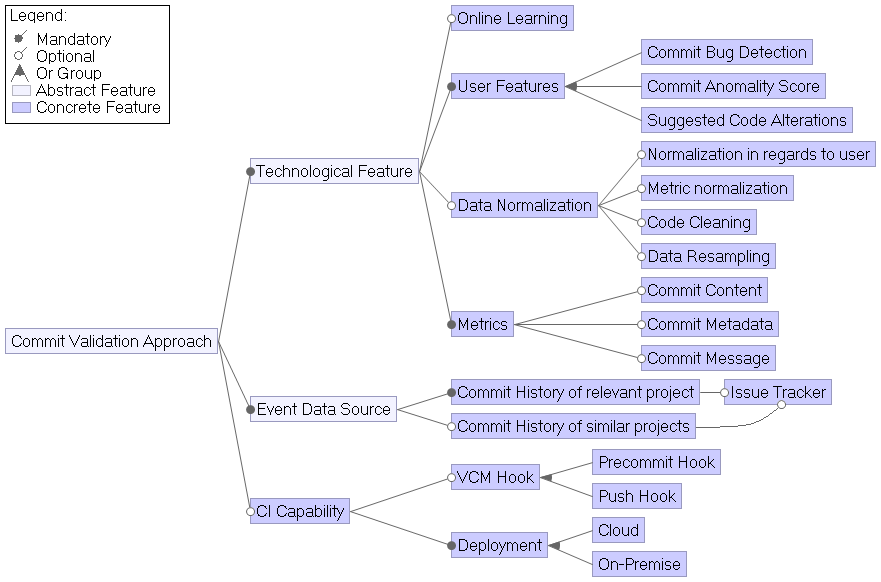
\includegraphics[width=15cm]{images/featuremodel}
	\caption{Featuremodel for Commit Validation approaches.}
	\label{fig:featuremodel}
\end{figure}

%Three categories have been specified for comparing Commit Validation approaches.
For comparing Commit Validation approaches the three categories Technological Features, Event Data Source and CI Capability have been defined.

The first category compares which \textit{Technological Features} approaches implement. The most important facet in this category is \textit{User Features}, which are features that are interesting to the end user of the approach. 
%Common user features are the detection of buggy commits and rating the anomality of commits.
More relevant to the performance of a method are the facets \textit{Metrics} and \textit{Data Normalization}. All approaches use some metrics to compare commit data, however the respectively used metrics vary between the approaches.
The latter facet shows which normalization techniques are used in the approaches to further improve their classification performance.
\textit{Online Learning} describes whether an approach is able to integrate analysis results made during production use into its analysis database, otherwise only the analysis results made on initial training data are considered. 

The \textit{Event Data Source} was also considered. This facet describes which sources of data are considered for training the classifier. All approaches are using the commit history of the repository for which new commits are being analyzed. Some approaches also used the commit history of similar repositories or issue trackers which belong to the repositories.
%TODO rename facettes in featuremodel from "...project" to "...repository". (oder doch einfach so lassen?)

Finally, the \textit{Capability for Continuous Integration} (or CI Capability) was considered. Because this paper focuses on Commit Validation, it is important how such an approach can be integrated into the commit process. As described in section \ref{sec:cvprocess}, VCM hooks are typical integration methods. The deployment of approaches is also interesting for practical usage, as a cloud based solution can be incompatible with company guidelines.
%TODO if more text is needed, go into detail which kinds of hooks can be used

%\begin{itemize}
%	\item Describe how relevant approaches differ from each other.
%	\item Derive list of criteria to compare Commit Validation approaches. For each criterium (roughly in one paragraph):
%	\begin{itemize}
%		\item Explain the criterium and what it means.
%		\item Discuss how the criterium is measured and derived from an Commit Validation approach.
%		\item Highlight the importance of this criterium in respect to comparing Commit Validation approaches.
%		\item Describe use cases for which this criterium is relevant.
%	\end{itemize}
%\end{itemize}

\subsection{Search Process}
\label{sec:searchprocess}
%\begin{itemize}
%	\item Describe why CLEVER was used as starting point for research for this paper. \cite{Nayrolles2018}
%	\item Describe how other approaches have been found based on CLEVER and how they match the papers scope as described in \ref{sec:scope}.
%\end{itemize}

The initial starting point of research for this work was the Commit Validation approach CLEVER developed by Nayrolles et.~al.~\cite{Nayrolles2018}. CLEVER suits the criteria defined in section \ref{sec:scope} of being a Just-in-Time Fault Detection program that uses software commits as primary mechanism and as such resembles a reference approach for the topic.  

To find more suitable approaches, backwards Snowball Sampling was performed on CLEVER \cite{10.2307/2237615}. A forward search did not yield results as CLEVER was still a very recent work at the time of this writing.

The paper by Nayrolles backwards referenced the papers by Kamei and Rosen, the latter introduced Commit Guru. Kamei's work was identified to be one of the first approaches on this topic and was included in this comparison due to its early release~\cite{Kamei2013}. Rosen's Commit Guru also very much fits the criteria, but differs from the other papers because it was released as a freely usable Open-Source project and as such is a very interesting work to consider~\cite{Rosen2015}. Yang's Deeper is a similar approach which builds upon the work of Kamei, but uses different internal mechanics and according to their statement was the first approach to use a deep neural network for classification~\cite{Yang2015}. Finally, the approach Unusual Commits by Goyal et. al. was considered because its scope differs from the other techniques by focusing more on the abnormality of commits rather than a binary classification into buggy or not, and similarly to Commit Guru, it was released as Open Source~\cite{Goyal2017}.

\subsection{Threats to Validity}
%\begin{itemize}
%	\item Discuss if there can be any biases when choosing and comparing Commit Validation approaches (See \cite{Kitchenham2004}).
%	\item Describe how this paper made sure not to be biased.
%\end{itemize}

A primary threat to the validity of this paper was due to the fact that it was written in a low effort seminar by a single person and thus included less research effort than in similar papers, thus a complete research of the scientific area was out of scope. State of the Art research principles such as Snowball Sampling as described in section \ref{sec:searchprocess} and a low yet for the research field representative sampling size were used to still give a qualitative overview of Commit Validation techniques \cite{10.2307/2237615}.

A possible Selection Bias towards Nayrolles' approach CLEVER can be attributed because it was selected as starting point for this research and because it is the most recent publication~\cite{Nayrolles2018}. This is also due to the novelty of the research area. Approaches differing from typical Commit Validation techniques such as Unusual Commits by Goyal et. al. were taken into consideration to counter this bias~\cite{Goyal2017}.

Another clear issue with the novelty of the research area is that not many papers were released which published openly usable and verifiable programs. Unusual Commits and Commit Guru were the only approaches that made their software Open Source, most other papers do not publish their software due to either academic or company guideline reasons. This not only applies to the papers mentioned in this work, but also to many others on the topic of Just-in-Time Fault Detection, such as the programs iFixR and Getafix mentioned in section~\ref{sec:scope}~\cite{Koyuncu2019,Bader2019}. This makes complete and unbiased performance reviews even with more research effort hard to realize. This work tries to still give insights into the performance of Commit Validation techniques by stating the comparisons given in the papers which introduce the respective techniques. Because no performance information was available for Unusual Commits, this also introduces an Attribution Bias~\cite{Goyal2017}.

As this paper only attempts to give an overview of the topic of Commit Validation, it hopefully still succeeds in doing so without in-depth performance benchmarks. However, this is a relevant topic for future work, as, in time, more openly usable programs will emerge and more research papers on their performance will be published.


%* This paper was developed by a single person with low research effort, but I followed sota research principles (snowballing).
%* Thus a complete research of the field was out of scope. But a small yet high-variety subset of approaches was considered to cover many branches of the field.
%* The topic is still emerging, many approaches do not offer freely usable and verifiable programs, but existing performance information in previous papers were considered and as much available information was taken into account. A complete performance review makes sense as future research project when more projects emerge and become freely available.
%(regarding the previous point:) * comparing the performance between CLEVER, Deeper, Kamei and Commit Guru would create a performance bias because the performance comparisons cannot be compared with each other. Considering only the performance data seperately without considering the performance of Unusual Commits creates an Attrition Bias. Because this comparison seeks to only give an overview of the topic, it hopefully still succeeds in doing that?
%* Possible bias towards CLEVER as that was the starting point and the most recent approach (Selection Bias). However approaches were taken into account that do differ from CLEVER in various aspects such as Deeper or Unusual Commits.



\section{Comparison of Commit Validation Approaches}
\label{sec:comparison}

With the comparison scheme described in the previous section,
%While the previous section has described the comparison scheme, 
the results will now be presented. 
%Section [TODO] specified categories with which the selected commit validation approaches have been categorized.
The five approaches have been ordered into one of three categories. Methods that only rely on analysis of metric data are reported on in section \ref{sec:comparison-metricbased}, methods that additionally employ machine learning techniques are described in section \ref{sec:comparison-ml}, and finally, the usage of code matching to further improve classification performance is described in section \ref{sec:comparison-codematching}.
The results are then presented in tabular form in table \ref{tab:classification}.

%TODO use \paragraph{title} per approach
\subsection{Purely Metric Based Approaches}
\label{sec:comparison-metricbased}

The approaches \textit{Commit Guru} by Rosen et. al. \cite{Rosen2015}, \textit{Unusual Commits} by Goyal et. al. \cite{Goyal2017} and the approach by Kamei et. al. \cite{Kamei2013} fall into the category of purely metric based approaches. They rely only on metrics that were directly derived from commits and use them to rate commits based on that. While Commit Guru works for any kind of Git repositories, Unusual Commits only works for repositories hosted on GitHub. Kamei did not state any restrictions of such kind \cite{Kamei2013}.

Commit Guru and Unusual Commits both support online learning, thus every new commit after the initial training is taken into account for the analysis of later commits.
%Unusual Commits implemented more data normalization methods than Commit Guru. 
Unusual Commits also normalizes data in regards to user information by building a profile per project and per developer, thus user information is respected when analyzing commits, 
while Kamei mentioned that they were also using data resampling.
%Both approaches did not mention that any other normalization techniques were used.
The techniques also vary in their output: Unusual Commits is the only approach to not strictly categorize a commit as either buggy or not, instead it rates the likelihood that a commit is \textit{unusual}, thus it differs from previous commits. Commit Guru and Kamei's approach output the same information as all other approaches, which is said categorization as buggy or not.

Commit Guru and Unusual Commits both only use the past commit history of the project which is analyzed as their event data source, not any other data sources, whereas Kamei's approach also takes information from the issue system attached to the repository into account.
As Unusual Commits only measures the abnormality of commits, it does not need any data labeling specifying which past commits are buggy or not, the comparison of derived metrics of new commits with average values already shows results.
Commit Guru on the other hand analyzes commit messages to detect keywords such as \texttt{fix} or \texttt{bug} to identify fix-commits and then backtrack the latest commit before the fix that changed similar lines to find out when the matching bug was introduced. This allows Commit Guru to effectively find previous buggy commits without the need for an additional data source such as an issue system.

Commit Guru is implemented in Python while Unusual Commits is realized in Java and R. It is also worth mentioning that both Commit Guru and Unusual Commits implement a graphical user interface. 
Figure \ref{fig:ui} shows the UI's of them both. 

Commit Guru deploys a standalone web application which is built upon Google's Angular framework where one can see the classification results \cite{Rosen2015}. On its website \url{https://commit.guru} a Git repository URL can be entered to initialize the analysis. This repository will then be added to the ones continuously reanalyzed on changes and will be added to a list on the page. From there the analysis results can be opened as depicted in figure \ref{fig:ui-commitguru}, where the classification results for all commits as well as various metrics are listed. When new changes are detected on a repository, it is automatically reanalyzed and an E-Mail notification is sent as response to the event, thus it shows CI capability in form of a Push Hook.

Unusual Commits on the other hand does not deploy its own webpage, but integrates into the GitHub web frontend, which causes the aforementioned restriction of only working with GitHub repositories \cite{Goyal2017}. The integration is realized by a Google Chrome plugin which can be installed from the Chrome Extension store\footnote{\url{https://chrome.google.com/webstore/detail/unusual-commits/hncljhkoaognphcmhdelchclkogepnae}}. Figure \ref{fig:ui-unusualcommits-history} shows how the calculated abnormality scores for each commit are embedded into GitHub's commit history. Their colors indicate the abnormality, giving the user a good overview at a glance. While no kind of CI capability is realized as new commits are only analyzed by actually visiting the commit history page, it still integrates well into a typical developer's workflow as this page is commonly visited to get an overview of changes made in the repository. 

When clicking on a commit in GitHub, a detail overview of it is opened. Unusual Commits also embeds information on this page as depicted in figure \ref{fig:ui-unusualcommits-details}. Here the abnormal facts are listed for this commit which justify the generated abnormality score.

%Unusual Commits is implemented as a Google Chrome plug-in which embeds classification results into the commit history on GitHub, while Commit Guru runs in a web application that lists the analysis results for a selected repository. It also listens to new commits, automatically reanalyzes them and sends E-Mail notifications in response to the event, thus it shows CI capability in form of a Push Hook. 
%Unusual Commits does not support any CI capabilities. 
Both are realized as free-to-use cloud applications.
Unlike Commit Guru and Unusual Commits, Kamei did not publish an openly usable program, thus their CI capability or any technological information cannot be reported on.

Kamei's approach and Commit Guru use the same set of metrics, which are metrics regarding the commit content such as changed lines of codes or the number of changed files, as well as the commit history, such as the commit purpose and information about the developer. Unusual Commits also considers the commit content, but instead of the latter metrics the commits metadata is taken into account.

Classification approaches that rely on purely metric based methods generally show high potential and are well represented in the research area. However, the availability of metrical vectors extracted from commit data also offers the usage of machine learning methods to further increase classification performance. The next section will detail the use of machine learning in existing Commit Validation approaches.


\begin{figure}[p!]
	\centering
	
	\begin{subfigure}[t]{\textwidth}
		\centering
		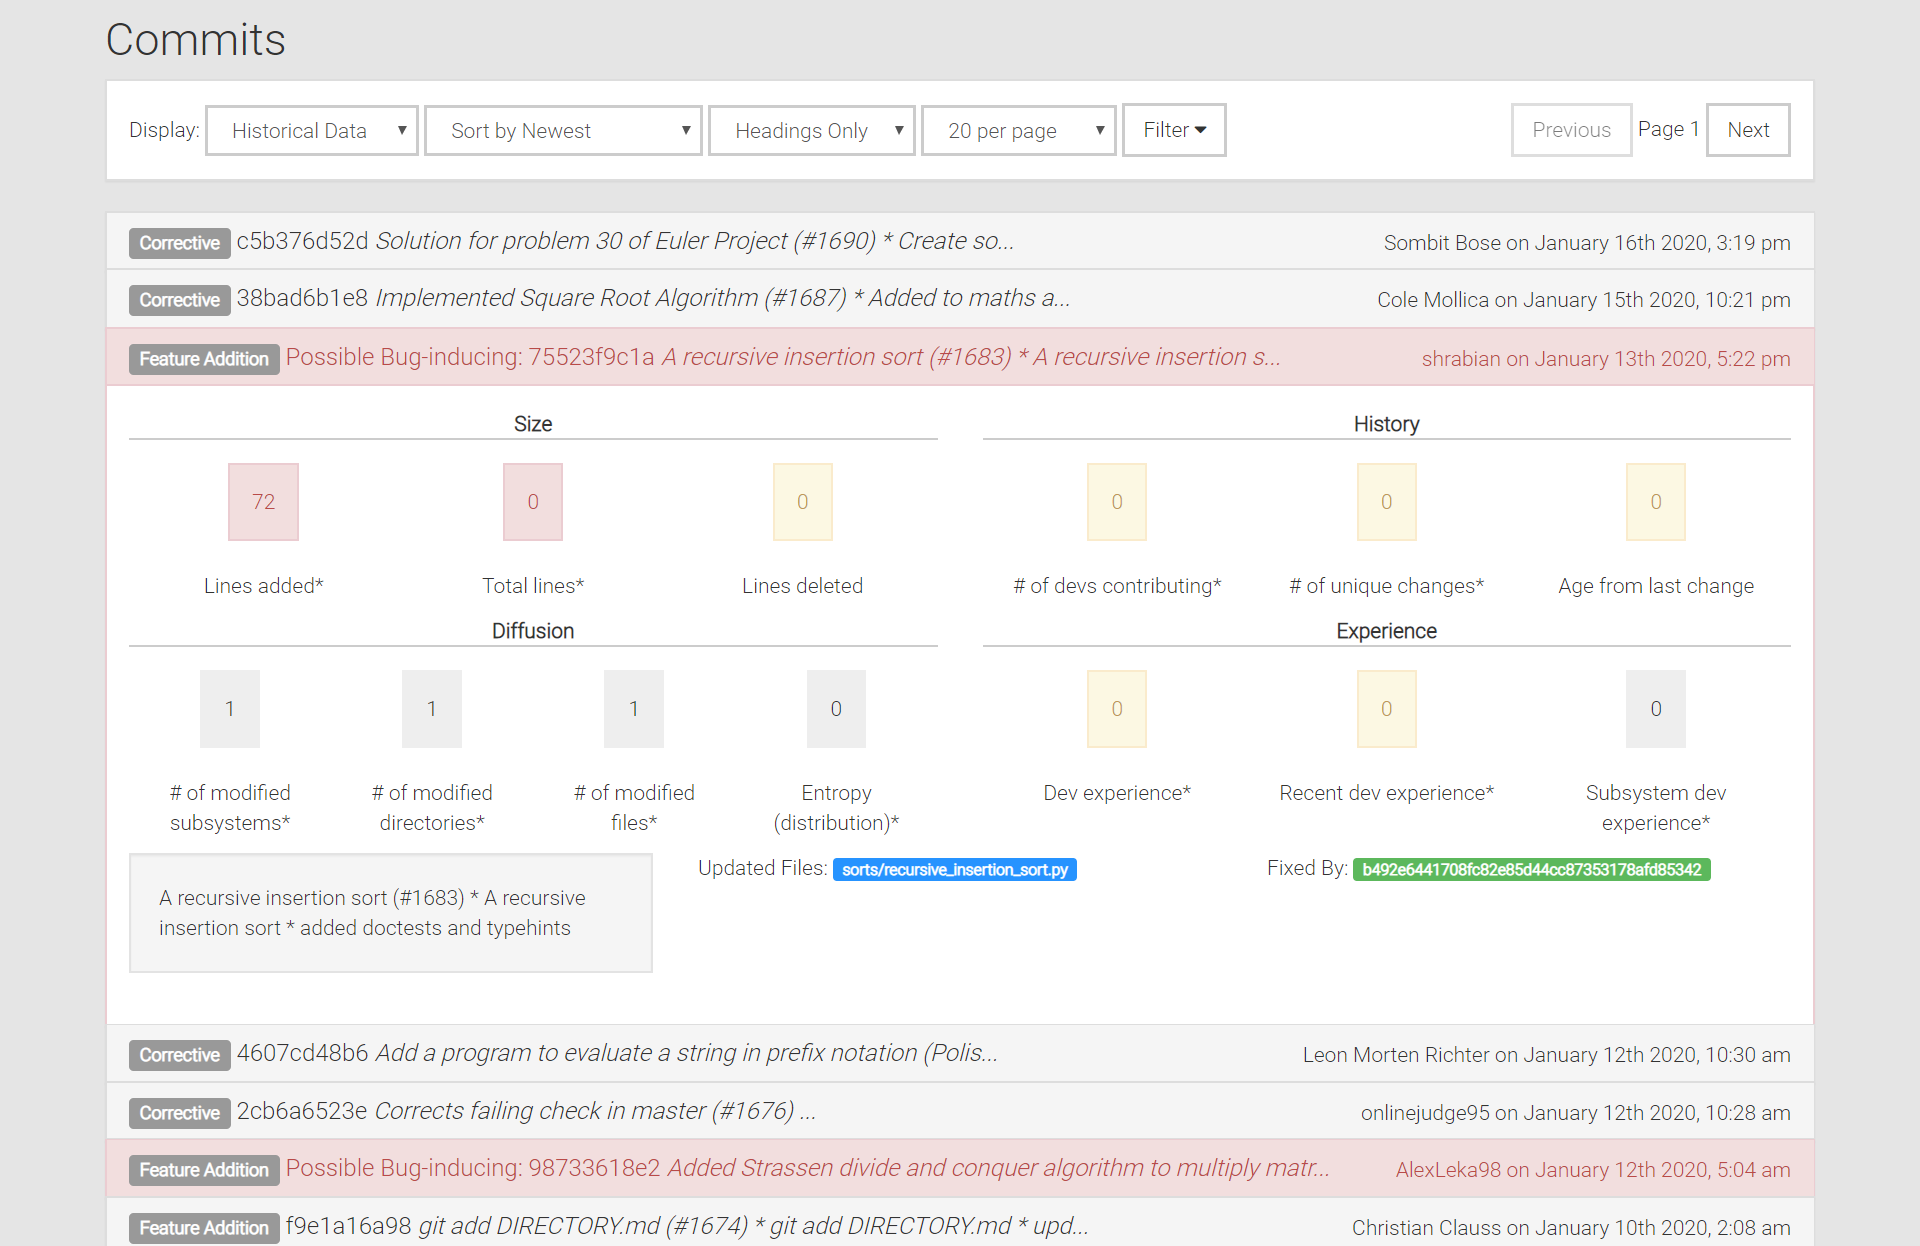
\includegraphics[width=.75\textwidth]{images/ui/commitguru/screenshot-repo-commits-buggy-smaller}
		\caption{Web panel of Commit Guru \cite{Rosen2015}. A dedicated page lists all commits of a repository and shows their classification result.}
		\label{fig:ui-commitguru}
	\end{subfigure}
	
	\begin{subfigure}[t]{.75\textwidth}
		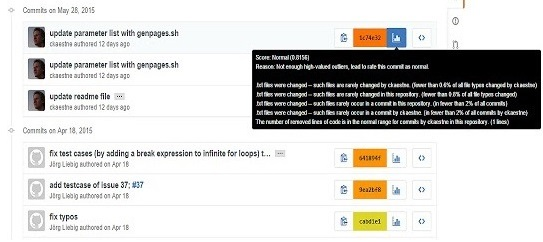
\includegraphics[width=\textwidth]{images/ui/unusualcommits/github-integration2-smaller}
		\caption{Unusual Commit embeds commit's abnormality scores in GitHub's commit history \cite{Goyal2017}.}
		\label{fig:ui-unusualcommits-history}
	\end{subfigure}
	
	\begin{subfigure}[t]{.75\textwidth}
		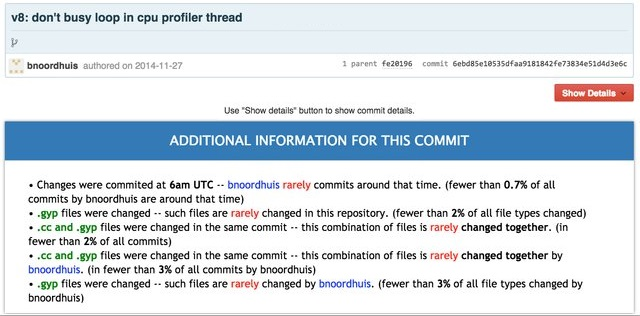
\includegraphics[width=\textwidth]{images/ui/unusualcommits/commit-details-smaller}
		\caption{When opening a commit, Unusual Commit describes why a potentially high abnormality score was calculated \cite{Goyal2017}.}
		\label{fig:ui-unusualcommits-details}
	\end{subfigure}
	\caption{Graphical user interfaces of Commit Guru \cite{Rosen2015} and Unusual Commits \cite{Goyal2017}}
	\label{fig:ui}
\end{figure}

%Both approaches considered the metrics which regard the content of the commits, such as changed lines of code or the number of changed files. Commit Guru also considered the history of the commit, its purpose and information about the authoring developer, while Unusual Commits considered the length of the commit message, the time of commit and the changed file types. \cite{Rosen2015,Goyal2017}

%\subsection{Results for Approaches Based on Anomaly Detection}
%%TODO (TODO: I'm not sure yet if anomaly-based approaches differ from metric-based approaches enough to justify an additional subsection)
%\begin{itemize}
%\item Describe the results for approaches based on anomaly detection such as UnusualCommit (\cite{Goyal2017}).
%\end{itemize}

\subsection{Approaches Based on Machine Learning}
\label{sec:comparison-ml}
%\begin{itemize}
%\item Describe the results for machine learning approaches.
%\end{itemize}

This category describes approaches which use machine learning techniques to increase evaluation performance.
While both Deeper by Yang \cite{Yang2015} and CLEVER by Nayrolles \cite{Nayrolles2018} implement such techniques, according to Yang et. al. Deeper was the first Just-in-Time Fault Detection approach to leverage deep neural networks for improved classification performance. Nayrolles' CLEVER on the other hand additionally implemented code matching alongside a machine learning model and will thus be described in more detail in section \ref{sec:codematching}.

Deeper was developed primarily in a research context and builds off the work of Kamei's approach \cite{Kamei2013}, successfully attempting to increase its classification performance with the new neural network. Due to the scientific background of the paper, online learning is not supported by Deeper. Typical methods common in machine learning such as data normalization and resampling are used. As most approaches Deeper only supports Commit Bug Detection without special features like the abnormality score supplied by Unusual Commits \cite{Goyal2017}. It also uses the most common data sources for training its model, which are the past commit history of the project for which new commits are being analyzed alongside an external issue system. Likely inspired by Kamei's work, it also uses the same metrics for classification, which regard the commits content and message. 

It is easy to see that Deeper is similar to Kamei's work in many aspects, which is not surprising because the primary contribution of Yang's paper was the integration of the neural network instead of Kamei's purely metric based method and 
due to their shared motivation by a scientific rather than an industrial context.
%because both are motivated by a scientific rather than an industrial context.

%TODO change if author responds
Information about the technical internal platform or the CI capability was not reported on by the original paper by Yang. They did however mention that they used a deep belief network algorithm to build a set of features and performed logistic regression on that.

While research shows that machine learning can increase performance in contrast to naive metric based methods, Nayrolles mentioned approach of code matching introduces a very different method for better classification results \cite{Nayrolles2018}. The next section will detail the use of code matching methods.

% Deeper by Yang and CLEVER by Nayrolles both use such techniques \cite{Nayrolles2018, Yang2015}. It is worth to mention that CLEVER also belongs to the next category of approaches based on Code-Matching.

%CLEVER is designed to work in production context inside Ubisoft where is was developed, while Deeper was developed in a research context. Thus CLEVER supports Online-Learning while Deeper does not. CLEVER stands out as the only approach which not only offers Bug Detection, but also Code Altering Suggestions, and as such also normalizes code syntax while Deeper does not. \cite{Nayrolles2018, Yang2015}

%When considering the Event Data Source, CLEVER also stands out here. While both use the commit history of the project on which commits are analyzed on as well as the associated issue tracker, CLEVER also takes the commit history of similar projects into account \cite{Nayrolles2018, Yang2015}. Nayrolles et. al. describes how the dependencies between projects are analyzed to calculate a measure of similarity for distinct projects \cite{Nayrolles2018}.

%\todo{Technical platform and CI Capability if/when author of Deeper answers.}

%They both use the same set of metrics when comparing commits, which are metrics considering the commit content such as changed lines of code or the changed number of files, and information about the 
%commit message %TODO other description for this metric category?
%such as the commit history or the purpose of the commit \cite{Nayrolles2018, Yang2015}.

\subsection{Approaches Based on Code Matching}%TODO bindestrich?
\label{sec:codematching}
\label{sec:comparison-codematching}
%\begin{itemize}
%\item Describe the results for machine learning approaches.
%\end{itemize}

Being published in 2018, Nayrolles' CLEVER was the most recent approach and implements features which none of the other publications do \cite{Nayrolles2018}. CLEVER is the only one which not only detects buggy commits, but also automatically generates suggested alterations for fault locations based on previous fixes in the commit history. While it uses past commits from the relevant project and the affiliated issue system in a similar way as other approaches do to detect faults, CLEVER is also the only approach to leverage commit data from similar projects. Nayrolles reported in his paper how dependency information of projects is used to cluster them based on their similarity.

The metrics used do not vary much from the ones used by other approaches. CLEVER's model was built on the foundation of Commit Guru and uses the same metrics as they do. However, as section \ref{sec:performance} detailing the performance of the approaches will show, CLEVER significantly outperforms Commit Guru. According to Nayrolles' paper, this is caused by its code matching component. This attempts to reduce the number of false-positives which is higher in other approaches and results in better precision.

In CLEVER, commits are first analyzed by a machine learning model, and only after positive classification code matching is performed to revalidate the likelihood of a fault. The code matching component expands the changeset of a commit to both of its sides to extract a complete syntactically correct code block. This code block is then compared to historically known defect introducing commits. For the comparison of code blocks, text-based clone detection techniques are used.

Nayrolles reported that just resorting to the code matching method and refrain from using the metric based classifier entirely would not yield any noticeable performance loss. The main reason why the metric based model is used prior to code matching is efficiency, as code matching is much more time consuming than the metric based analysis.

With the code matching analysis results linking a similar bug introducing commit, the generation of altered code suggestions is almost a trivial process: the fix commit for the bug is determined using the issue system, and the fix changeset is adapted to the new code context by changing indentation depth and variable names.

In contrast to other approaches, CLEVER was motivated by an industrial rather than a scientific context. It was developed for production use within Ubisoft with a company-internal deployment planned. Because of that, its online learning and Continuous Integration capabilities are both important and were both implemented. On the latter one, Nayrolles et. al. decided on precommit hooks which run directly on the developers machines at the moment they commit source code, resulting in fast feedback.


\subsection{Performance Comparison}
\label{sec:performance}

When comparing Commit Validation approaches, the evaluation performance is an important point to consider. Due to the effort of this work and the fact that not all approaches are publicly available, an objective performance evaluation on all five approaches on a consistent dataset was out of scope for this paper. However, Nayrolles et. al. included an objective performance comparison between their approach and Rosen's approach \cite{Nayrolles2018}. In the same 
way, %TODO wording?
Yang et. al. included a performance comparison between their approach and Kamei's \cite{Yang2015}. While both surveys use different datasets and thus cannot be compared to with each other, they give insights into how CLEVER compares to Commit Guru and how Deeper compares to Kamei's approach in regards to evaluation performance.

Table \ref{tab:perfclever} describes the findings from Nayrolles' paper \cite{Nayrolles2018}, while table \ref{tab:perfdeeper} describes those from Yang's paper \cite{Yang2015}.

Nayrolles findings show that his approach performs better than Commit Guru, with an precision increase of more than $13\%$ and an increase in the F1 measure of about $7\%$. Yang also found that his approach performs better than the one described by Kamei, with which he compared with in his paper. Even though the performance gap was not as noticeable in his case (with an increase of the F1 measure of only about $1\%$), there was still an improvement. 

It is also notable that Nayrolles approach primarily improved precision compared to Commit Guru, while Deeper improved recall compared to Kamei's approach. 
A likely cause for this is Nayrolles' implementation of code matching, which reduced the number of false positives, resulting in better precision.
%A likely cause for this are differing training settings, as increasing the precision in model training often leads to worse recall and vice versa. 

% MOVED INTO DISCUSSION
%It is also notable that Nayrolles approach primarily improved the precision compared to Commit Guru, while Deeper improved the recall compared to Kamei's approach. A likely cause for this are differing training settings, as increasing the precision in model training often leads to worse recall and vice versa. However the more interesting correlation from the numbers suggests that establishing machine learning methods brings noticeable performance improvements compared to relying solely on metric-based techniques. Nayrolles also reported that incorporating code matching significantly increases performance in CLEVER \cite{Nayrolles2018}.

\begin{table}[t]
	\centering
	\caption{Performance comparison of CLEVER and Commit Guru, as evaluated by Nayrolles et. al. \cite{Nayrolles2018}}
	\begin{tabular}{@{}lrr@{}}
		\toprule
		& \multicolumn{1}{l}{CLEVER} & \multicolumn{1}{l}{Commit Guru} \\ \midrule
		Precision  & 79.10\%                    & 66.71\%                         \\
		Recall     & 65.61\%                    & 63.01\%                         \\
		F1 measure & 71.72\%                    & 64.80\%                         \\ \bottomrule
	\end{tabular}
	% TODO precision is avg precision
	\label{tab:perfclever}
\end{table}

\begin{table}[t]
	\centering
	\caption{Performance comparison of Deeper and Kamei's approach as well as a standard Logistic Regression, denoted as LR. The comparison was evaluated by Yang et. al. \cite{Yang2015}}
	\begin{tabular}{@{}lrrr@{}}
		\toprule
		& \multicolumn{1}{l}{Deeper} & \multicolumn{1}{l}{Kamei} & \multicolumn{1}{l}{LR} \\ \midrule
		Precision  & 35.64\%                    & 35.71\%                   & 59.92\%                \\
		Recall     & 69.03\%                    & 65.52\%                   & 18.28\%                \\
		F1 measure & 45.06\%                    & 43.91\%                   & 25.30\%                \\ \bottomrule
	\end{tabular}
	\label{tab:perfdeeper}
\end{table}


%\begin{itemize}
%	\item Show Performance comparison tables
%	\item Describe tables
%\end{itemize}

\subsection{Comparison Results}
%\begin{itemize}
%	\item Table mapping all metrics/criteria (described in \ref{sec:scheme}) and all 5 approaches to results.
%\end{itemize}

The aforementioned results have been collected in Table \ref{tab:classification} where each of the described facets map to specific values per identified Commit Validation approach. The basic structure of the table maps to the feature model described in figure \ref{fig:featuremodel}. 

%TODO change if authors answer
Cells marked with \textit{N/A} indicate that the respective information was not mentioned in the reporting paper. While I have tried to contact the authors of Deeper and Kamei's approach, they could not be reached for further details. The technical platform was also hard to determine for many papers that only reported on the classification model, even though it would be interesting to know as it can influence the practicality of integrating the system in production environments. Only Commit Guru and Unusual Commits have reported on their platform as they were also the only approaches that published their source code as open source.

%\begin{figure}[H]
%	\centering
%	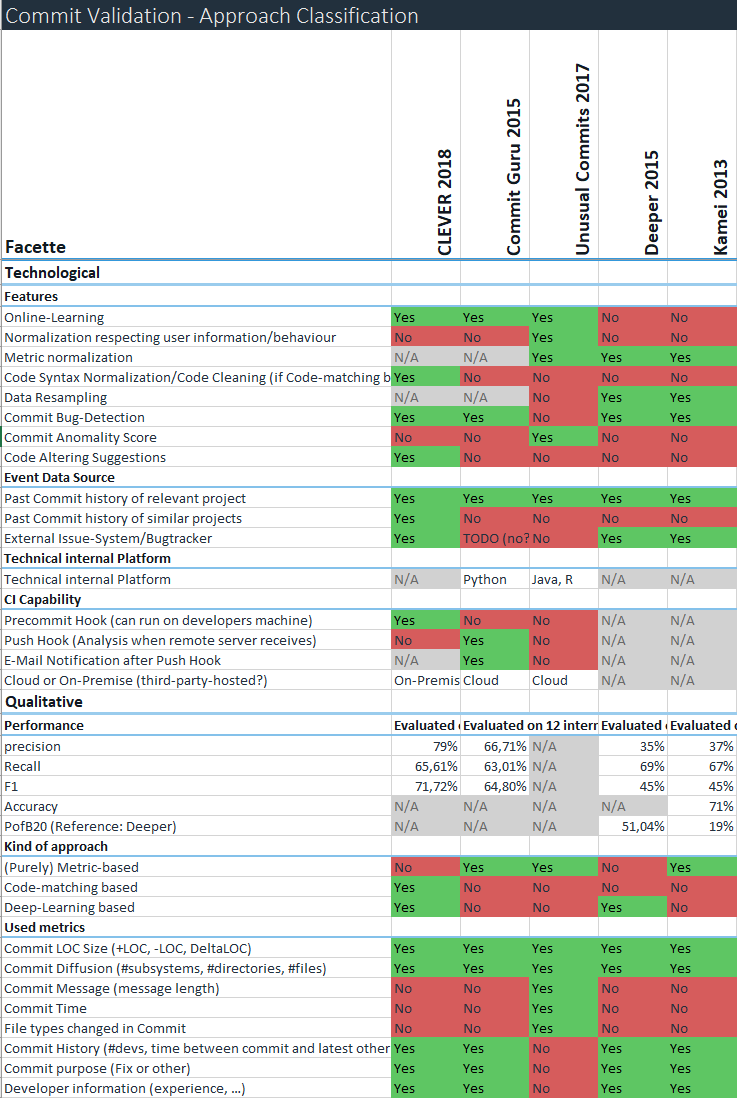
\includegraphics[width=15cm]{images/classification}
%	\caption{Classification results [TODO]}
%	\label{fig:classification}
%\end{figure}

\begin{table}[t]
	\centering
	\caption{Classification results of the five identified approaches: CLEVER by Nayrolles \cite{Nayrolles2018}, Commit Guru by Rosen \cite{Rosen2015}, Unusual Commits by Goyal \cite{Goyal2017}, Deeper by Yang \cite{Yang2015}, Kamei's approach \cite{Kamei2013}.}
	\begin{tabular}{@{}llllll@{}}
		\toprule
		& CLEVER     & Guru   & Unusual & Deeper & Kamei \\ \midrule
		\textit{User Features}             &            &        &         &        &       \\ 
		Online Learning                    & Yes        & Yes    & Yes     & No     & No    \\
		Normalization to user information  & No         & No     & Yes     & No     & No    \\
		Metric normalization               & N/A        & N/A    & Yes     & Yes    & Yes   \\
		Code Cleaning and Matching         & Yes        & No     & No      & No     & No    \\
		Data Resampling                    & N/A        & N/A    & No      & Yes    & Yes   \\
		Commit Bug Detection               & Yes        & Yes    & No      & Yes    & Yes   \\
		Commit Abnormality Score           & Yes        & Yes    & No      & Yes    & Yes   \\
		Suggestions of Code Alteration     & Yes        & No     & No      & No     & No    \\ \midrule
		\textit{Event Data Source}         &            &        &         &        &       \\ 
		Commit history of relevant project & Yes        & Yes    & Yes     & Yes    & Yes   \\
		Commit history of similar projects & Yes        & No     & No      & No     & No    \\
		External Issue-System              & Yes        & No     & No      & Yes    & Yes   \\ \midrule
		\textit{Technical background}      &            &        &         &        &       \\ 
		Technical internal Platform        & N/A        & Python & Java, R & N/A    & N/A   \\ \midrule
		\textit{CI Capability}             &            &        &         &        &       \\ 
		Precommit Hook                     & Yes        & No     & No      & N/A    & N/A   \\
		Push Hook                          & No         & Yes    & No      & N/A    & N/A   \\
		E-Mail Notification                & N/A        & Yes    & No      & N/A    & N/A   \\
		Cloud or On-Premise                & On-Premise & Cloud  & Cloud   & N/A    & N/A   \\ \midrule
		\textit{Considered Metrics}        &            &        &         &        &       \\ 
		Commit Content                     & Yes        & Yes    & Yes     & Yes    & Yes   \\
		Commit Metadata                    & No         & No     & Yes     & No     & No    \\
		Commit Message                     & Yes        & Yes    & No      & Yes    & Yes   \\ \bottomrule
	\end{tabular}
	\label{tab:classification}
\end{table}

\section{Discussion of Comparison Results}
\label{sec:discussion}
%\todo{
%\begin{itemize}
%	\item Emphasize interesting findings from the results.
%	\item Describe how performance was evaluated on the approaches and how their performance can be compared.
%	\item Describe how the specified categories of Commit Validation techniques can be mapped to use cases.
%	\item Outline how this mapping can be used to find an suitable Commit Validation technique for a new project.
%\end{itemize}
%}

When considering the classification results in table \ref{tab:classification}, various interesting findings can be deduced. In the following section, notable correlations will be emphasized and their possible causes discussed.

All approaches supply some result to the user, either Commit Bug Detection where each commit is either marked as buggy or not, a score which rates the abnormality of commits in contrast to other commits, or automatically generated suggested alterations for possibly faulty code. Since a primary topic of Commit Validation lies in Fault Detection, the binary detection of bugs in commits is implemented by most approaches. Only Unusual Commits \cite{Goyal2017} generates an abnormality score which leaves the decision of whether a commit is actually faulty up to the user, only "strange" commits are highlighted to guide the user's focus.

CI Capability was a feature which was considered very important for this paper, however not many approaches actually implemented it. Especially among papers focused on research this was usually either not realized or not reported on, while performance was more emphasized. With more emerging papers on the topic of Commit Validation and increasing usage in industry, this capability is likely to be more broadly implemented in future methods.

The feature online learning correlates with whether a paper had a scientific goal or not. Deeper and Kamei's approach focused on evaluating Fault Detection methods by building respective classification models \cite{Yang2015, Kamei2013}, while CLEVER, Commit Guru and Unusual Commits implemented programs which were meant to be used in an industrial context \cite{Nayrolles2018,Rosen2015,Goyal2017}. In the first two approaches, only offline learning was established, thus they performed initial training on a dataset and then evaluated the resulting models.

One interesting finding comes from the numbers of the aforementioned performance comparisons, as both CLEVER and Deeper perform better than their reference approaches. They also implement similar methods as both rely on machine learning. This correlation suggests that establishing machine learning methods brings noticable performance improvements compared to relying solely on metric-based techniques. Nayrolles also reported that incorporating code matching significantly increases performance in CLEVER, which explains the major advantage it has in numbers compared to Commit Guru \cite{Nayrolles2018}.

The event data source is also closely related to the classification performance. Here CLEVER also stands out as it is the only approach to consider projects that are similar to the project for which commits are analyzed. The usage of previous Commit Data of the analyzed project are typical event sources which are used by all approaches. Incorporating data from issue systems also correlates with the performance increases and usually makes sense to do because issue systems are used in most industrial software engineering projects, thus their data is available anyway.

Another feature that likely affects classification performance is data normalization regarding user information and behavior, a feature which was only implemented by Unusual Commits \cite{Goyal2017}.
% TODO if this was not described before, describe here
Because no performance comparison of Unusual Commits was found, an implication of the positive or negative effect of this method cannot be concluded here, but it is an interesting finding nonetheless.

A topic closely related to the classification performance are the metrics which were taken into consideration during classification. Between most approaches, the used metrics did not differ too much: CLEVER, Commit Guru, Deeper and Kamei all used metrics regarding commit content and the commit message. Only Unusual Commits used commit metadata instead of the commit message. This suggests that a typical set of relevant metrics for defect detection has been established in the research area. The metrics were initially introduced by Kamei's original paper and referenced by the other papers, thus Kamei et. al. initially defined these relevant metrics and they were used mostly unchanged since \cite{Kamei2013}.




\section{Related Surveys on Commit Validation}
\label{sec:relatedsurveys}
%\begin{itemize}
%	\item Discuss and describe other surveys such as \cite{Kim2008,Catolino2019,Syed2019,Yang2016}.
%	\item Highlight for each survey how its scope differs from the scope of this paper.
%\end{itemize}

%There exist various studies and surveys 
Various studies and surveys exist
on the topic of either Commit Validation or Just-in-Time Defect Prediction. While some such as Catolino et. al. \cite{Catolino2019} and Syed \cite{Syed2019} took practical implementations into account, most focused on comparing the performance of underlying components such as the prediction model, resampling and ensemble learning methods or used set of metrics. For Catolino's and Syed's papers it is notable that both also referenced CLEVER and Commit Guru.

Kiehn et. al. reported on existing publications and developed a new classification model which extended the used metrics from previous approaches by new information based on code ownership and more, showing that code ownership can successfully be applied in change risk classification \cite{Kiehn2019}.

A similar focus on evaluating the underlying components of Commit Validation approaches was set by the study of Zhu et. al. \cite{Zhu2018}. They explored imbalance data handling methods such as resampling and ensemble learning to evaluate their performance effect in change classification. They found that a combination of ensemble learning and resampling shows better results than other methods. 

Similarly, Malhotra et. al. explored various machine learning methods to determine their overall predictive capability \cite{Malhotra2017}. According to them, their work confirms the overall predictive capability of all machine learning methods used in their research for defect prediction. This matches our suggestion made in section \ref{sec:discussion} that approaches which rely on machine learning yield better results than the ones that do not. They also highlighted that a single layered perceptron shows the best result as a machine learning method.

Finally, in a very early study almost five years before all other mentioned studies, Punitha and Chitra developed a novel approach for defect prediction which was based on three different classification methods, namely Support Vector Machine, Fuzzy Inference System and Genetic Algorithm \cite{Punitha2013}. They verified that the combination of these learners leads to a better prediction model.

All identified studies varied from the scope of this paper by focusing on the performance of defect classification. As mentioned, studies concentrating on user features and the practical use of Commit Validation methods are rare, especially because the research topic focuses on Fault Detection and less on the aspect of commits. Especially CI capability is a feature which was considered important for this paper, but was usually not taken into account by any of the studies.

%TODO %%%%%%%%%%%%%%%%%%%%%%%%%%%%%%%%%%%%%%%%%%%%%%%%%%%%%%%%%%%%%%%%%%%%%
%TODO %%%%%%%%%%%%%%%%%%%%%%%%%%%%%%%%%%%%%%%%%%%%%%%%%%%%%%%%%%%%%%%%%%%%%
%TODO %%%%%%%%%%%%%%%%%%%%%%%%%%%%%%%%%%%%%%%%%%%%%%%%%%%%%%%%%%%%%%%%%%%%%
%TODO %%%%%%%%%%%%                              %%%%%%%%%%%%%%%%%%%%%%%%%%%
%TODO %%%%%%%%%%%%    OWN PROOFREAD PROGRESS    %%%%%%%%%%%%%%%%%%%%%%%%%%%
%TODO %%%%%%%%%%%%                              %%%%%%%%%%%%%%%%%%%%%%%%%%%
%TODO %%%%%%%%%%%%%%%%%%%%%%%%%%%%%%%%%%%%%%%%%%%%%%%%%%%%%%%%%%%%%%%%%%%%%
%TODO %%%%%%%%%%%%%%%%%%%%%%%%%%%%%%%%%%%%%%%%%%%%%%%%%%%%%%%%%%%%%%%%%%%%%
%TODO %%%%%%%%%%%%%%%%%%%%%%%%%%%%%%%%%%%%%%%%%%%%%%%%%%%%%%%%%%%%%%%%%%%%%

\section{Conclusions}
\label{sec:conclusions}

%\subsection{Summary}
%\begin{itemize}
%	\item Give a short summary on the comparison scheme and which relevant criteria have been defined.
%	\item Highlight interesting findings that were derived from the comparison results.
%\end{itemize}

%\subsection{Contributions}
%\begin{itemize}
%	\item Highlight the contributions that the proposed comparison scheme did to the scientific topic of Commit Validation.
%	\item Discuss the relevance of the findings in regards to the scientific topic.
%\end{itemize}

%\subsection{Future Work}
%\begin{itemize}
%	\item Discuss relevant parts that have not been covered by this work.
%	\item Highlight next steps to conduct to improve results.
%\end{itemize}

%summary
The aim of this paper was to give an overview of the scientific topic of Commit Validation as well as existing works that have emerged in this area. In an effort to objectively compare and discuss differences between Commit Validation approaches, a feature model for such approaches was defined in section \ref{sec:scheme} and five relevant yet diverse methods were compared. The evaluation focused on CI capability and user features which both were considered important for the topic, but insights on the performance of said methods were given as well.

%contributions
The contributions of this paper include the basic introduction of Commit Validation, the definition an objective evaluation scheme to highlight differences between Commit Validation approaches and the comparison of the five mentioned approaches.

%summary
Interesting findings have shown that many differences in the classification approaches exist and affect their performance. It was also shown that on this novel topic many new publications and methods continue to emerge and new concepts and features are introduced. With it becoming more relevant in industrial contexts, production features such as CI capability and online learning are likely to be implemented more often as well. Especially the deployment of Nayrolles' CLEVER in Ubisoft is an important step of bringing the topic closer to industry \cite{Nayrolles2018}.

%future work
As the threats to the validity of this paper have shown, comparing the performance of Commit Validation methods continues to be a difficult objective with many approaches staying closed source and not being openly published, and with not many reports on the performance of programs available. This marks an important area for future research, with more emerging methods and papers. While the performance of programs seems not to be well covered yet, the performance of underlying components such as relevant machine learning models or similar supplies more papers and surveys, thus more research by involving these performance data can lead to more interesting findings.
